%%%%%%%%%%%%%%%%%%%%%%%%%%%%%%%%%%%%%%%%%%%%%%%%%%%%%%%%%%%%%%%%%%%%%%
% Overleaf (WriteLaTeX) Example: Molecular Chemistry Presentation
%
% Source: http://www.overleaf.com
%
% In these slides we show how Overleaf can be used with standard 
% chemistry packages to easily create professional presentations.
% 
% Feel free to distribute this example, but please keep the referral
% to overleaf.com
% 
%%%%%%%%%%%%%%%%%%%%%%%%%%%%%%%%%%%%%%%%%%%%%%%%%%%%%%%%%%%%%%%%%%%%%%

\documentclass{beamer}

\mode<presentation>
{
  \usetheme{Madrid}       % or try default, Darmstadt, Warsaw, ...
  \usecolortheme{default} % or try albatross, beaver, crane, ...
  \usefonttheme{default}    % or try default, structurebold, ...
  \setbeamertemplate{navigation symbols}{}
  \setbeamertemplate{caption}[numbered]
} 

\usepackage[english]{babel}
\usepackage[utf8x]{inputenc}
\usepackage{chemfig}
\usepackage[version=3]{mhchem}

\usepackage{hyperref}
  \hypersetup{colorlinks=true}
  \hypersetup{urlcolor=blue}
  \hypersetup{linkcolor = .}
\usepackage{xcolor}
\usepackage{siunitx}
  \sisetup{separate-uncertainty = true}
\usepackage{physics}
\usepackage[font=small,labelfont=bf]{caption}
\usepackage{subcaption}
\usepackage[en-GB]{datetime2}
\usepackage{overpic}
\usepackage{feynmp}
\DeclareGraphicsRule{*}{mps}{*}{}

\usepackage{scalerel}
\newcommand{\mylbrace}[2]{\vspace{#2pt}\hspace{6pt}\scaleleftright[\dimexpr5pt+#1\dimexpr0.06pt]{\lbrace}{\rule[\dimexpr2pt-#1\dimexpr0.5pt]{-4pt}{#1pt}}{.}}
\newcommand{\myrbrace}[2]{\vspace{#2pt}\scaleleftright[\dimexpr5pt+#1\dimexpr0.06pt]{.}{\rule[\dimexpr2pt-#1\dimexpr0.5pt]{-4pt}{#1pt}}{\rbrace}\hspace{6pt}}

% Here's where the presentation starts, with the info for the title slide
\title[BESIII Oxford]{BESIII Oxford Group Meeting}
\author{Martin Tat}
\institute{Oxford LHCb}
\date{28th April 2022}

\titlegraphic{
\includegraphics[width = 4cm, height = 2.8cm]{lhcb.jpg}\hspace{1cm}~%
              
\includegraphics[width = 4cm, height = 2.8cm]{bes3.jpg}}

\begin{document}

\begin{frame}
  \titlepage
\end{frame}

% These three lines create an automatically generated table of contents.
%\begin{frame}{Outline}
%  \tableofcontents
%\end{frame}

\section{Introduction}

\begin{frame}{Introduction}
  \begin{itemize}
    \setlength\itemsep{1.0em}
    \item{Previously:}
    \begin{itemize}
      \item{$F_+$ measurement of $D\to KK\pi\pi$}
      \item{$10$ CP tags and $K_{S, L}\pi\pi$ tags}
      \item{Peaking backgrounds}
    \end{itemize}
    \item{What has happend since?}
    \begin{itemize}
      \item{Presentation in Charm group 15th March 2022}
      \item{Reweighting of $KK\pi\pi$ model}
      \item{Toy studies}
      \item{Systematic uncertainties}
    \end{itemize}
  \end{itemize}
\end{frame}

\begin{frame}{Reweighting of \texorpdfstring{$KK\pi\pi$}{KKpipi} model}
  \begin{figure}
    \centering
    \begin{subfigure}{0.33\textwidth}
      \centering
      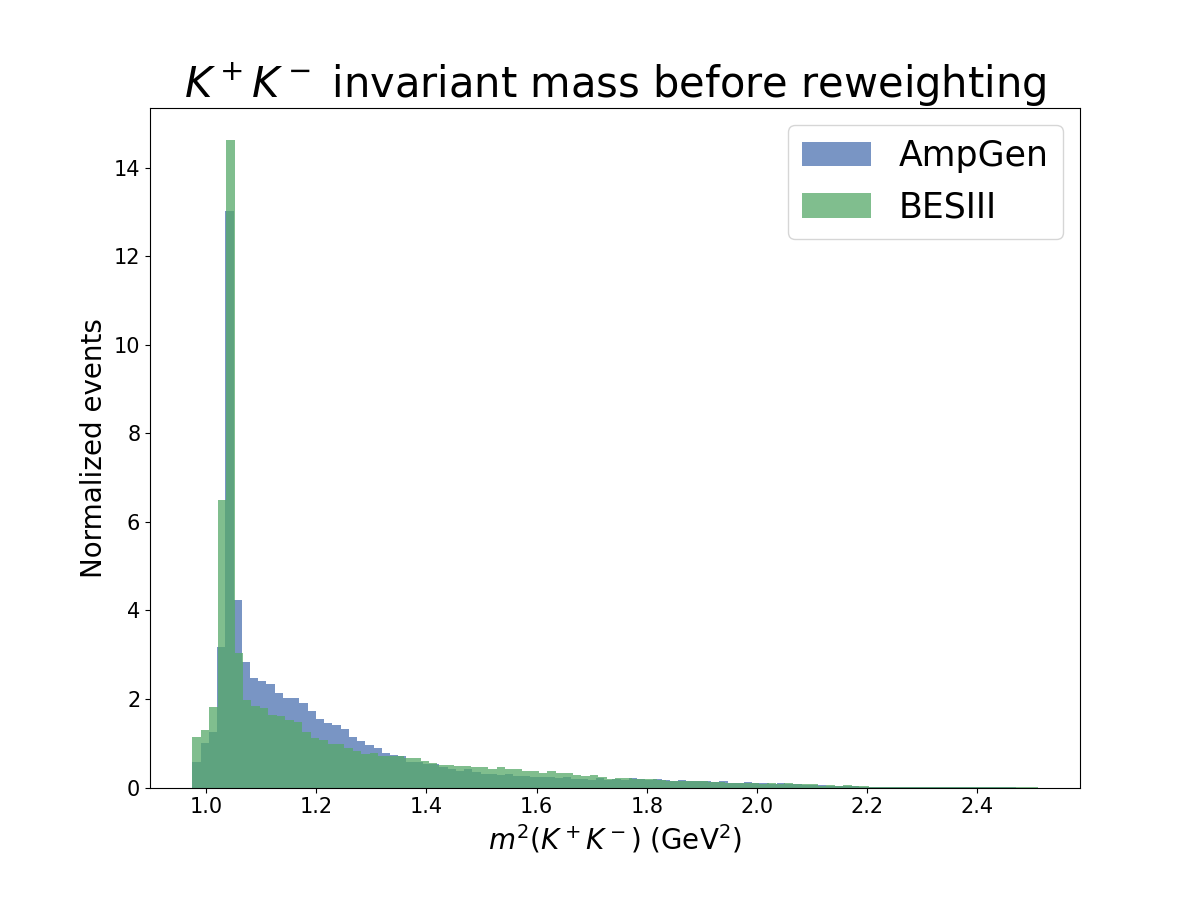
\includegraphics[width=\textwidth]{Plots/s01_BeforeReweighting.png}
      \caption{$K^+K^-$}
    \end{subfigure}%
    \begin{subfigure}{0.33\textwidth}
      \centering
      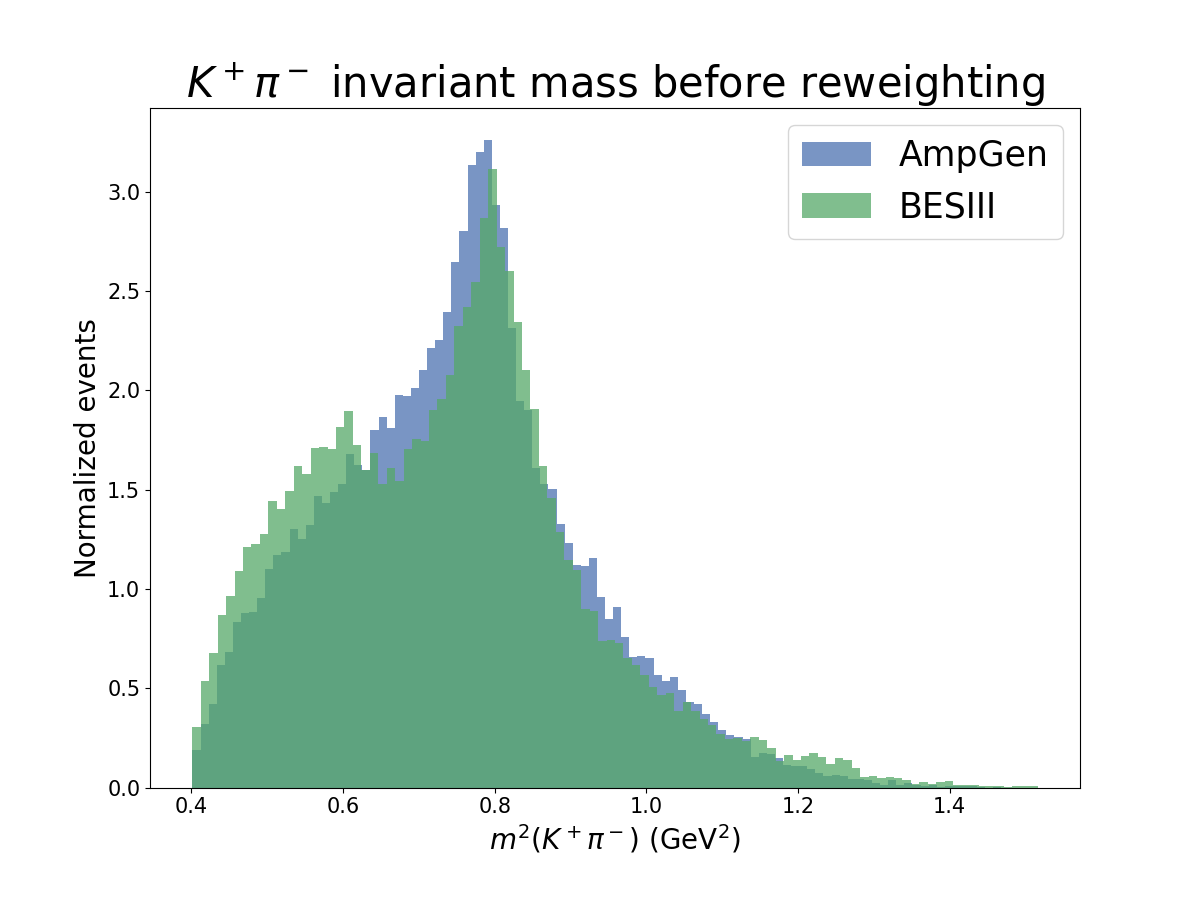
\includegraphics[width=\textwidth]{Plots/s03_BeforeReweighting.png}
      \caption{$K^+\pi^-$}
    \end{subfigure}%
    \begin{subfigure}{0.33\textwidth}
      \centering
      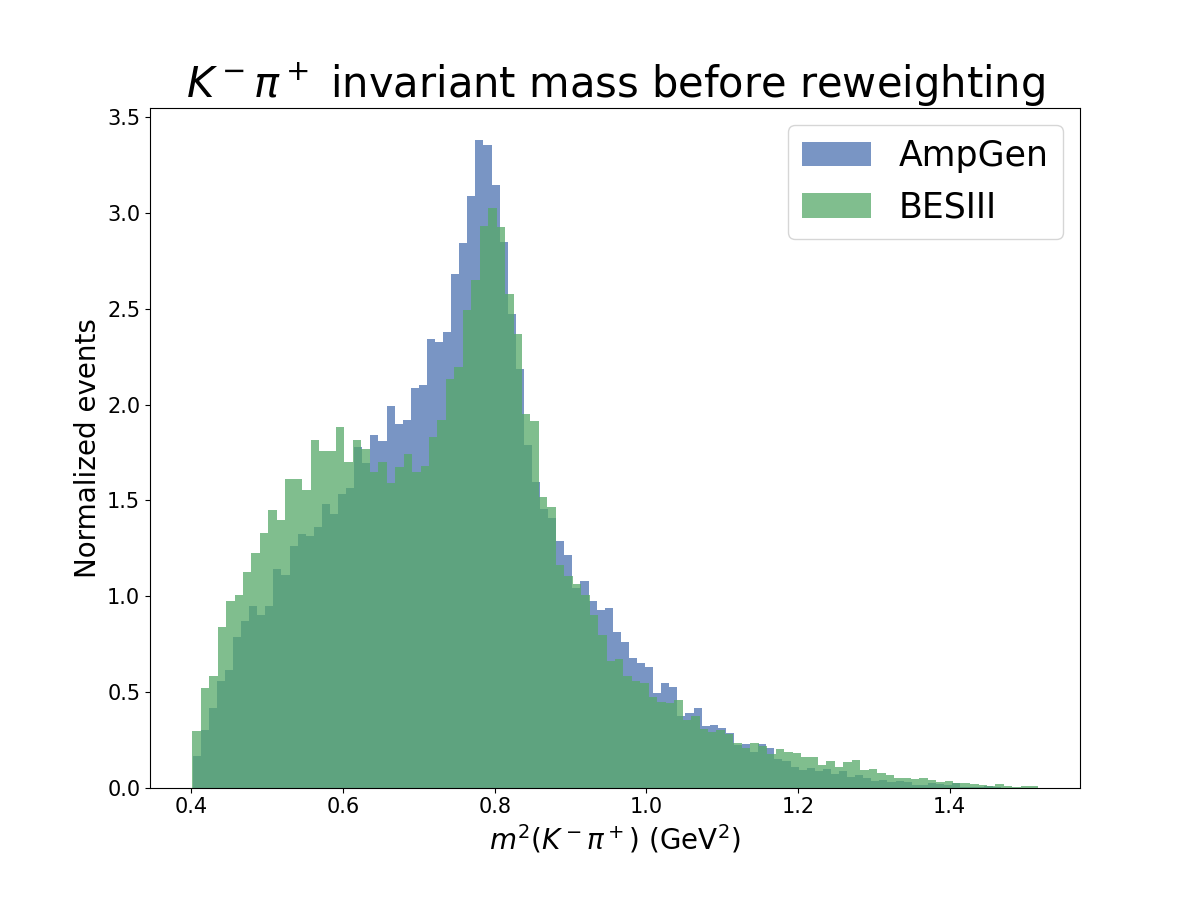
\includegraphics[width=\textwidth]{Plots/s12_BeforeReweighting.png}
      \caption{$K^-\pi^+$}
    \end{subfigure}
    \begin{subfigure}{0.33\textwidth}
      \centering
      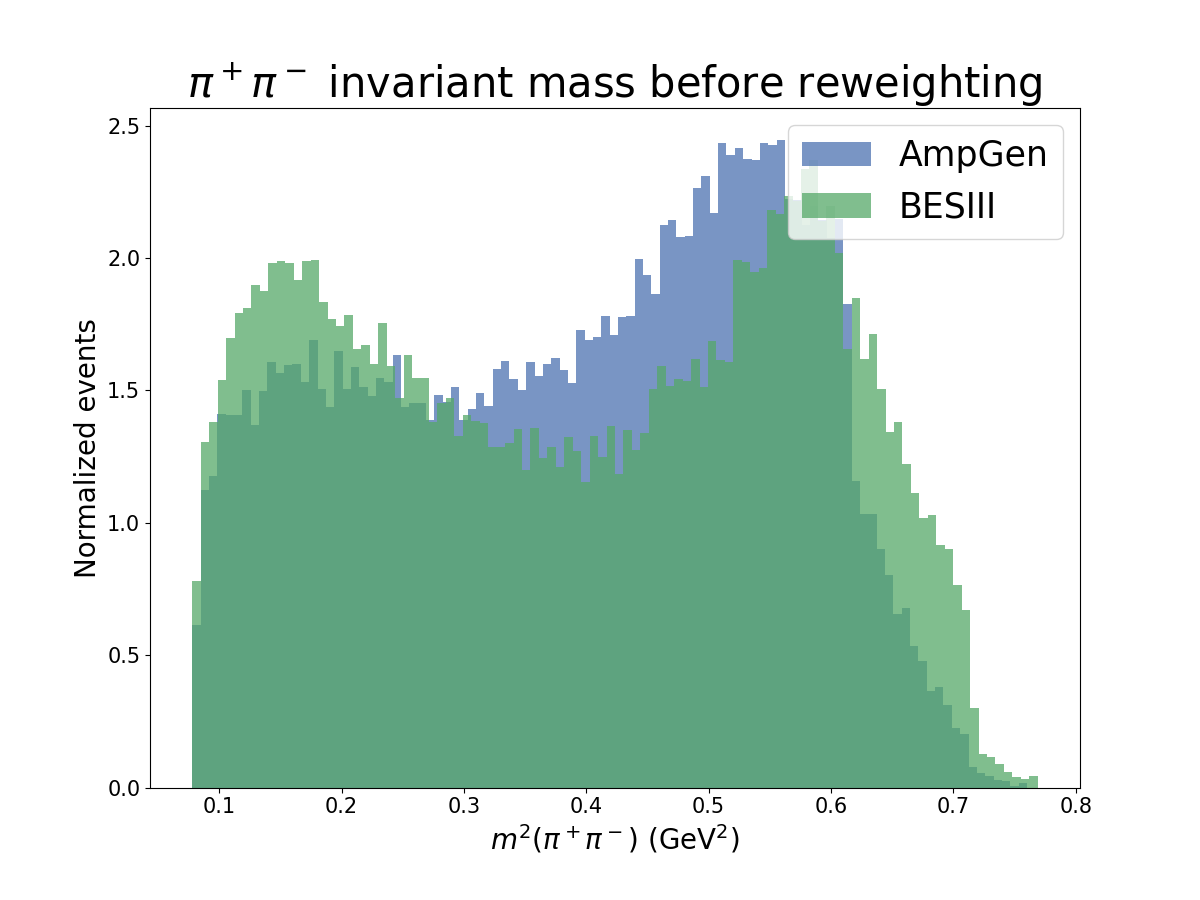
\includegraphics[width=\textwidth]{Plots/s23_BeforeReweighting.png}
      \caption{$\pi^+\pi^-$}
    \end{subfigure}%
    \begin{subfigure}{0.33\textwidth}
      \centering
      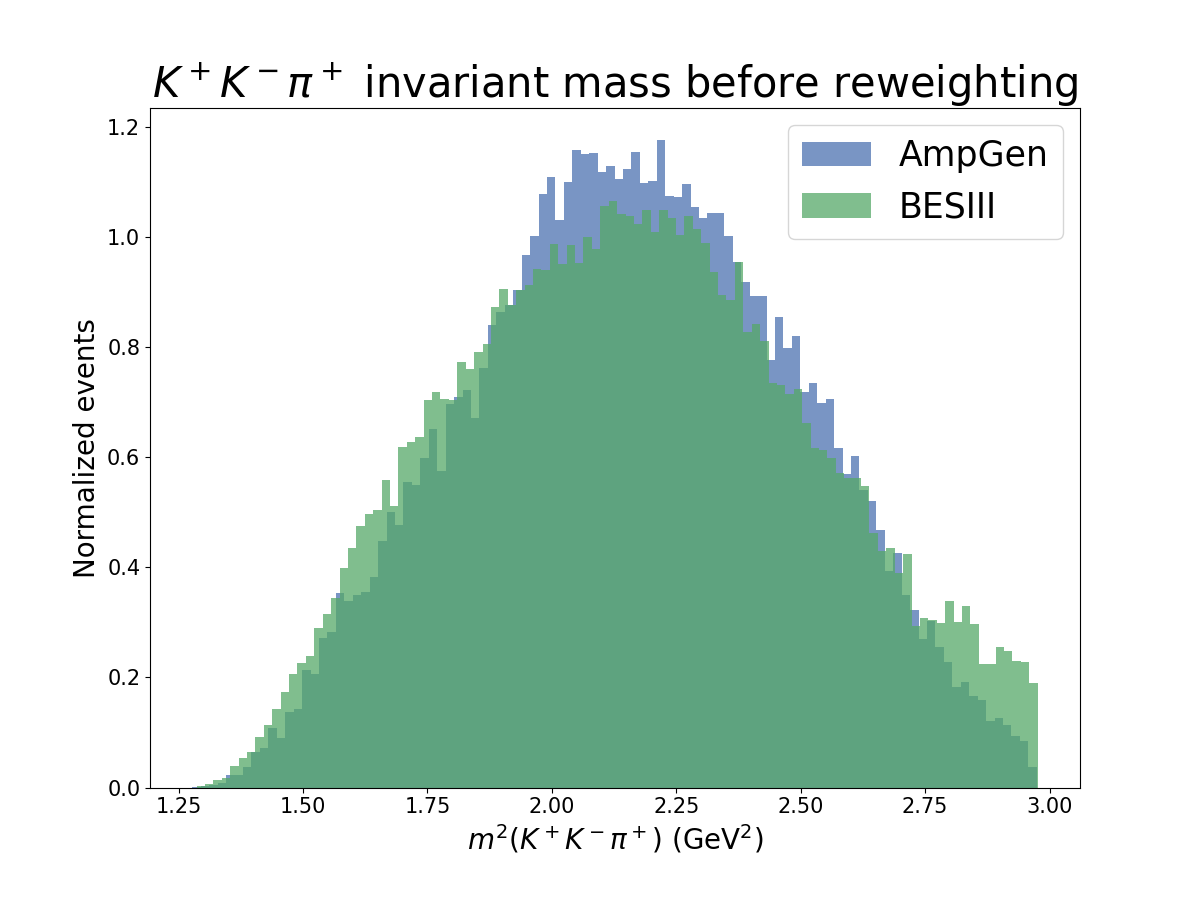
\includegraphics[width=\textwidth]{Plots/s012_BeforeReweighting.png}
      \caption{$K^+K^-\pi^+$}
    \end{subfigure}
    \caption{Before reweighting}
  \end{figure}
\end{frame}

\begin{frame}{Reweighting of \texorpdfstring{$KK\pi\pi$}{KKpipi} model}
  \begin{figure}
    \centering
    \begin{subfigure}{0.33\textwidth}
      \centering
      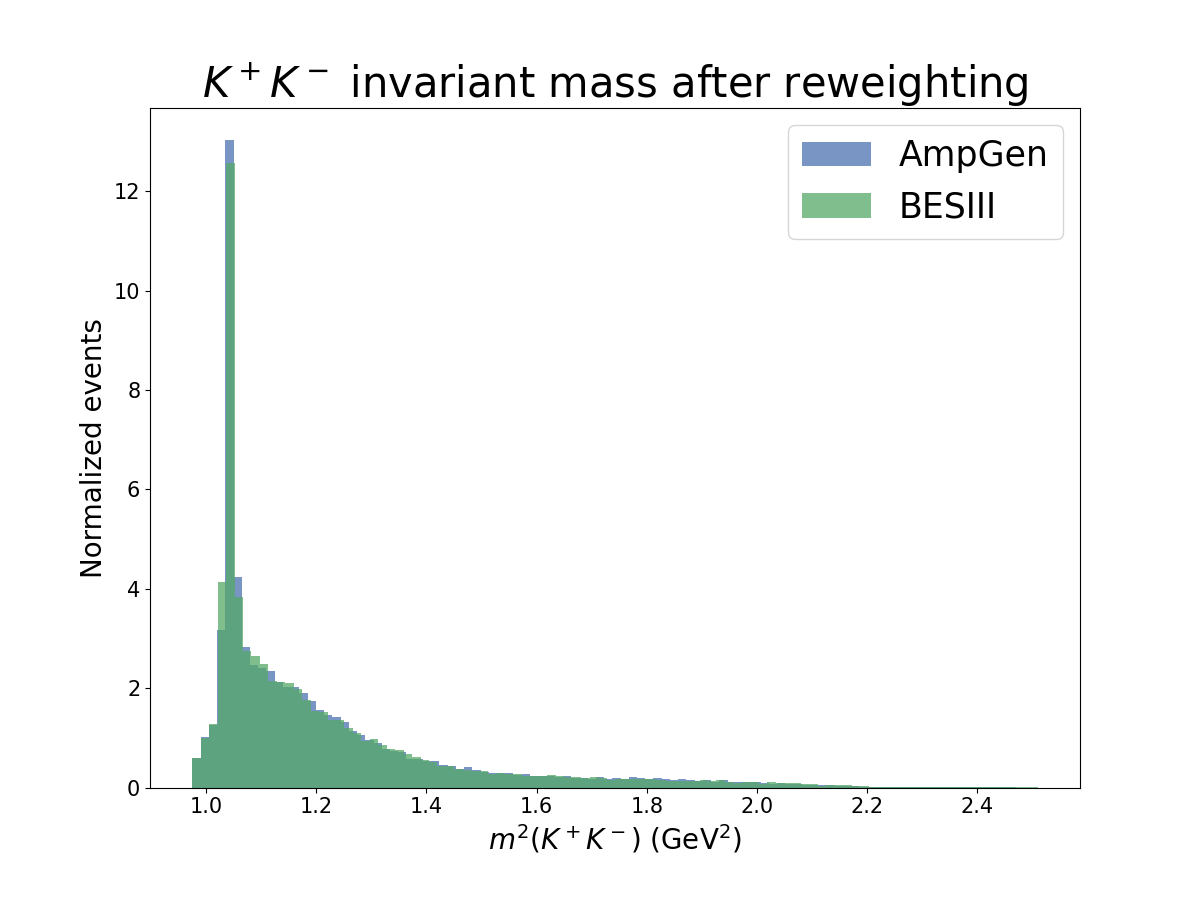
\includegraphics[width=\textwidth]{Plots/s01_AfterReweighting.png}
      \caption{$K^+K^-$}
    \end{subfigure}%
    \begin{subfigure}{0.33\textwidth}
      \centering
      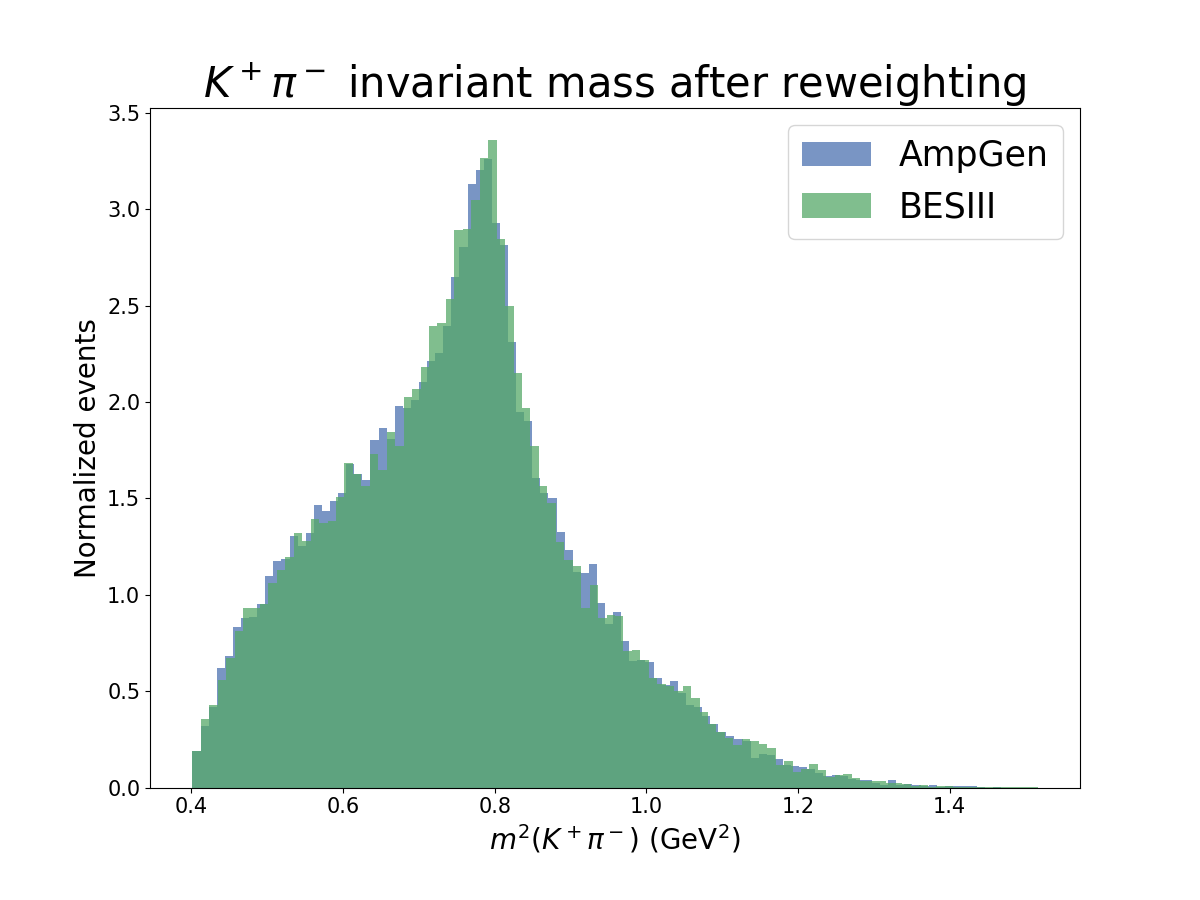
\includegraphics[width=\textwidth]{Plots/s03_AfterReweighting.png}
      \caption{$K^+\pi^-$}
    \end{subfigure}%
    \begin{subfigure}{0.33\textwidth}
      \centering
      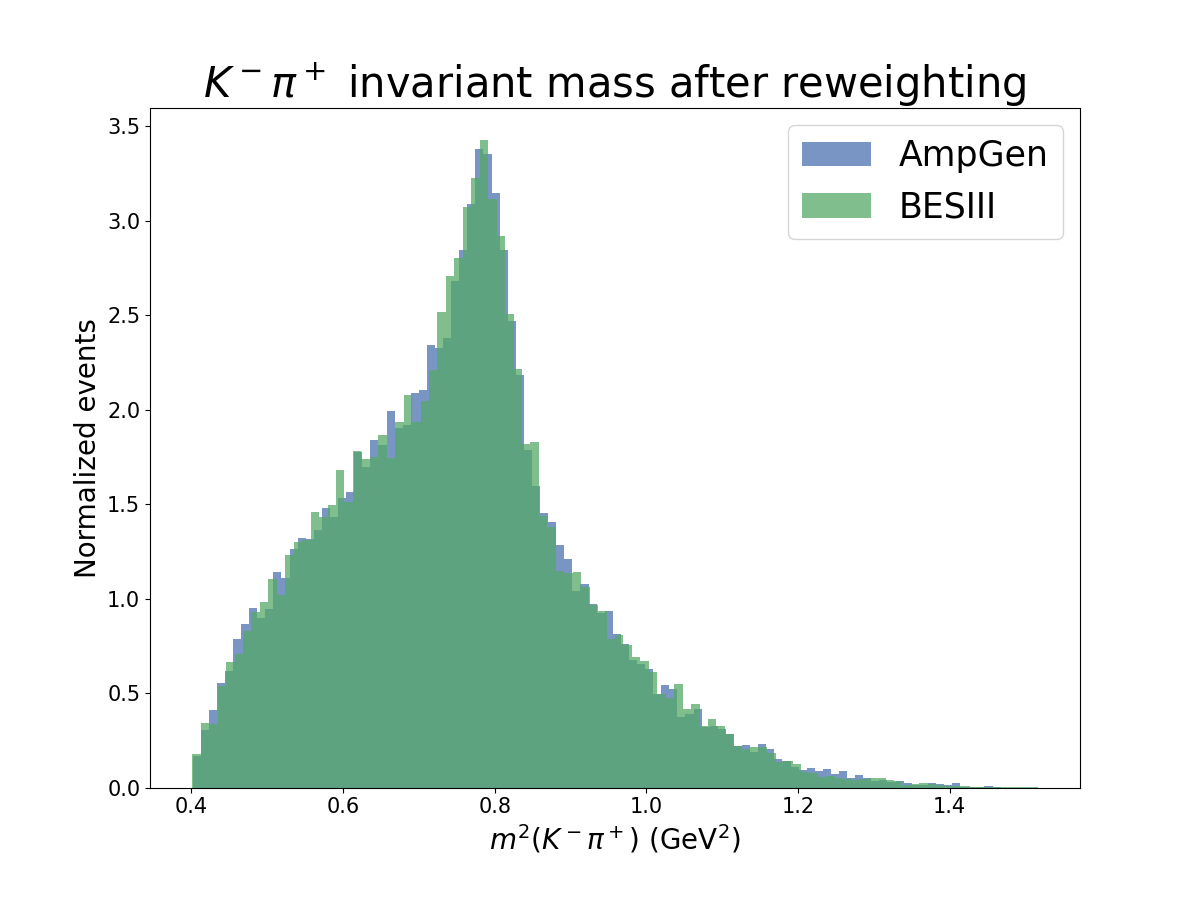
\includegraphics[width=\textwidth]{Plots/s12_AfterReweighting.png}
      \caption{$K^-\pi^+$}
    \end{subfigure}
    \begin{subfigure}{0.33\textwidth}
      \centering
      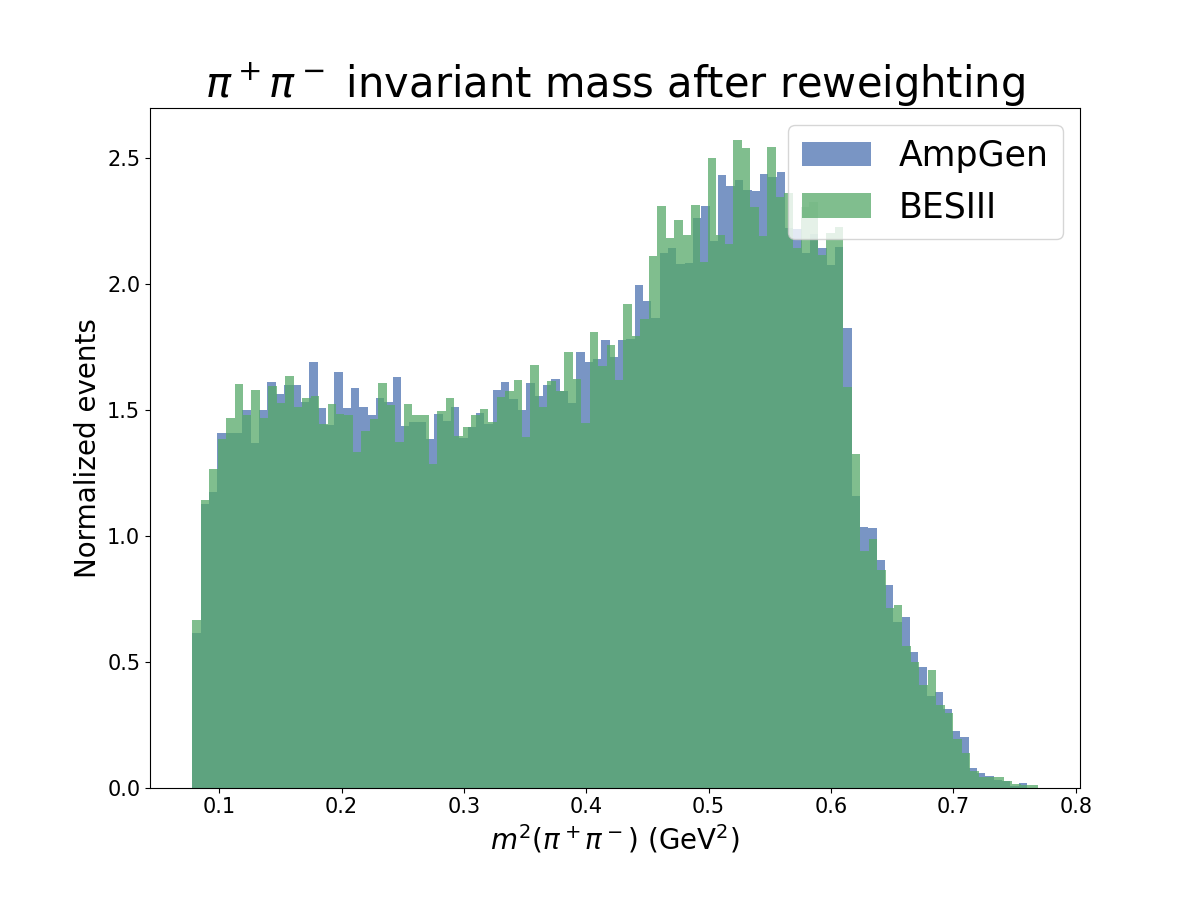
\includegraphics[width=\textwidth]{Plots/s23_AfterReweighting.png}
      \caption{$\pi^+\pi^-$}
    \end{subfigure}%
    \begin{subfigure}{0.33\textwidth}
      \centering
      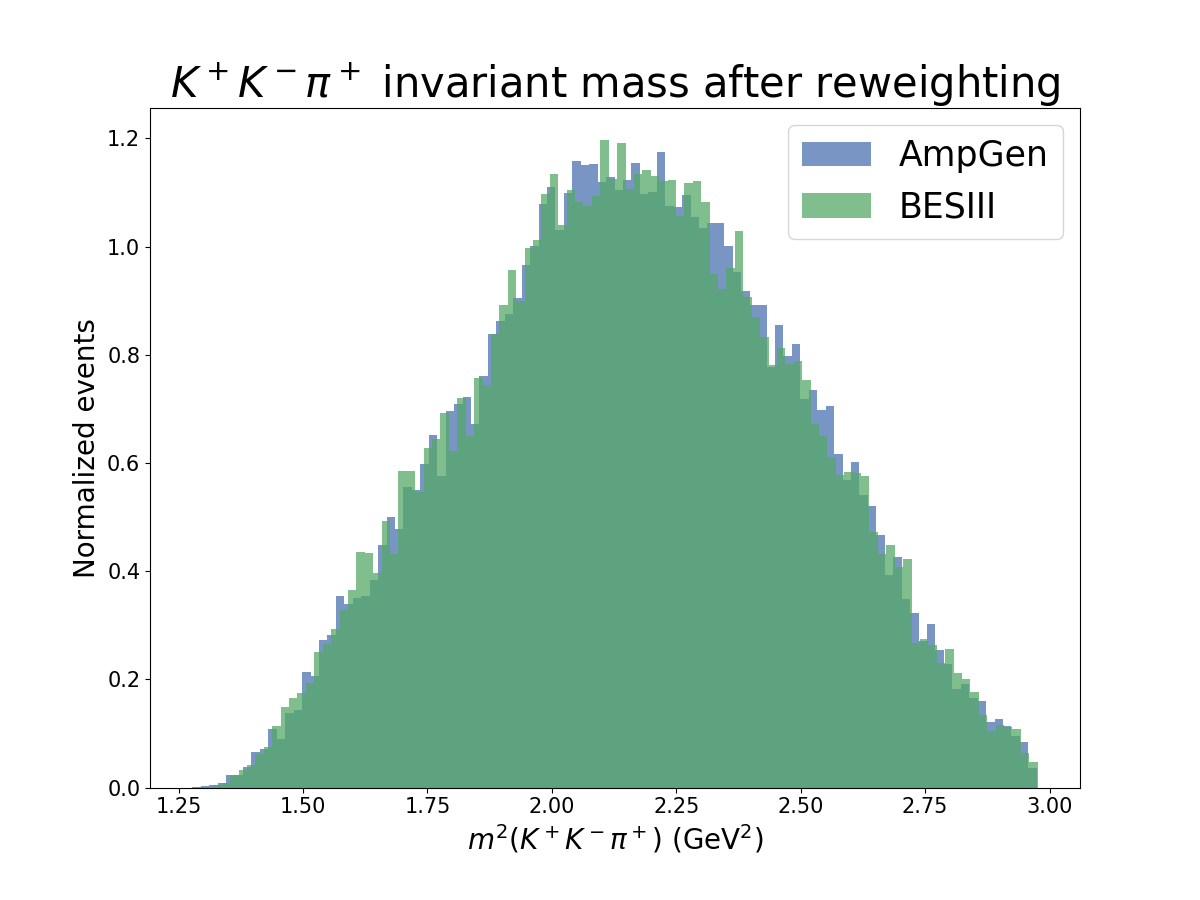
\includegraphics[width=\textwidth]{Plots/s012_AfterReweighting.png}
      \caption{$K^+K^-\pi^+$}
    \end{subfigure}
    \caption{After reweighting}
  \end{figure}
\end{frame}

\begin{frame}{Toy studies}
    \begin{figure}
    \centering
    \begin{subfigure}{0.33\textwidth}
      \centering
      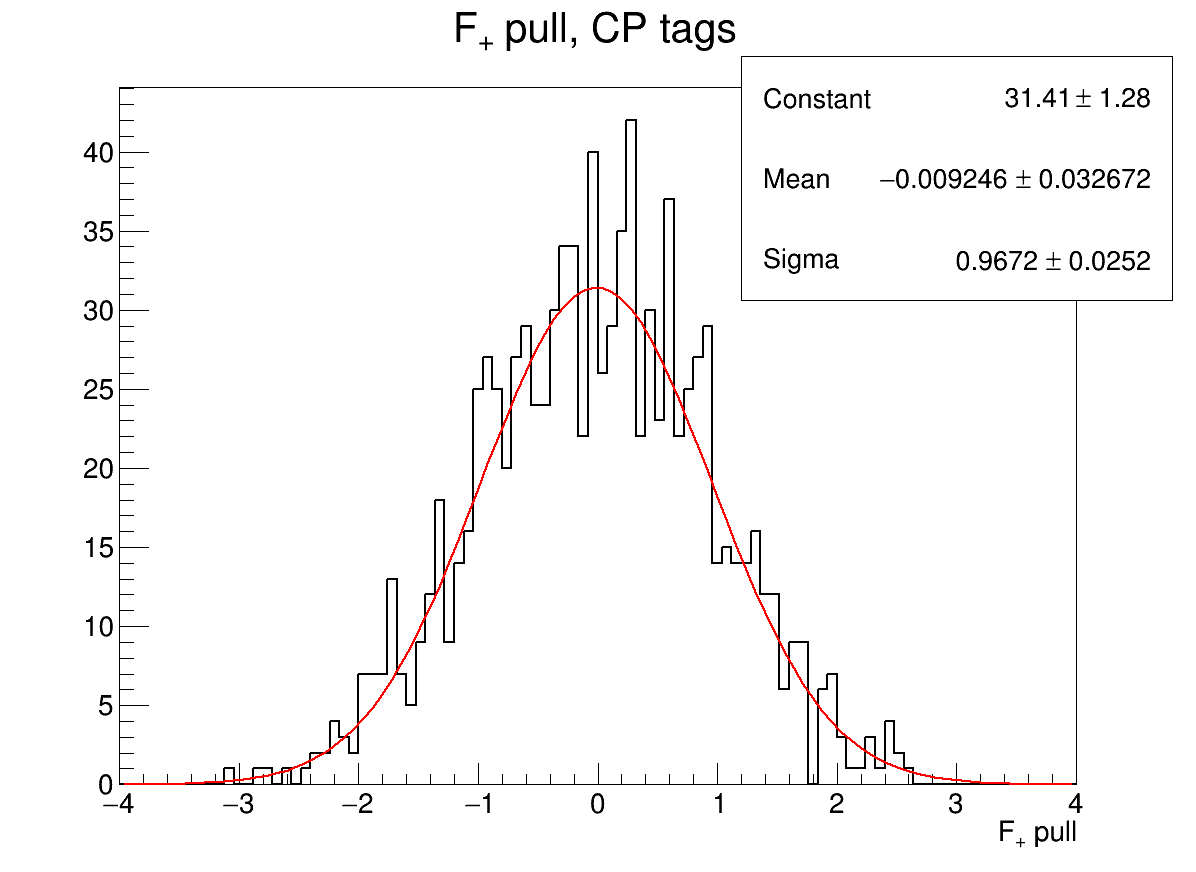
\includegraphics[width=\textwidth]{Plots/FPlus_toy_CP.png}
      \caption{CP tags}
    \end{subfigure}%
    \begin{subfigure}{0.33\textwidth}
      \centering
      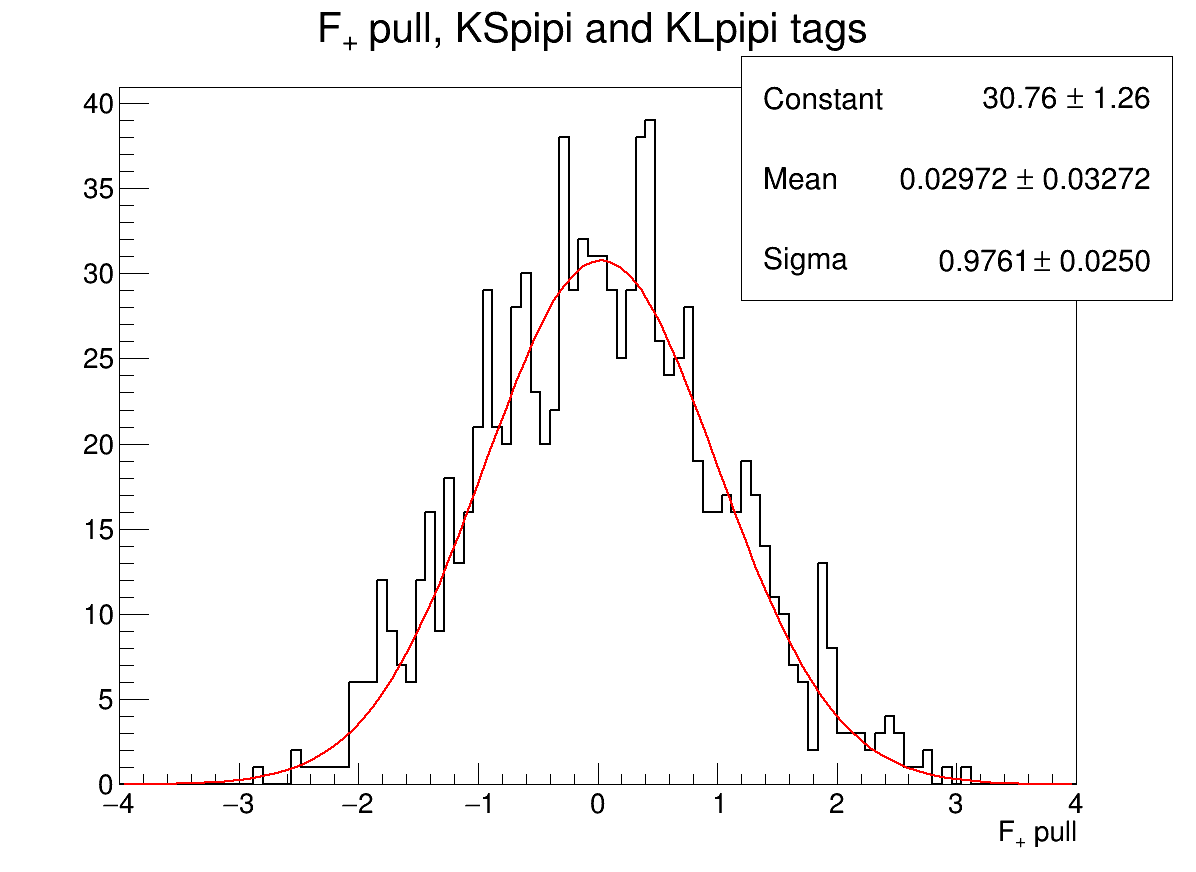
\includegraphics[width=\textwidth]{Plots/FPlus_toy_K0pipi.png}
      \caption{$K_{S, L}\pi\pi$ tags}
    \end{subfigure}
    \begin{subfigure}{0.33\textwidth}
      \centering
      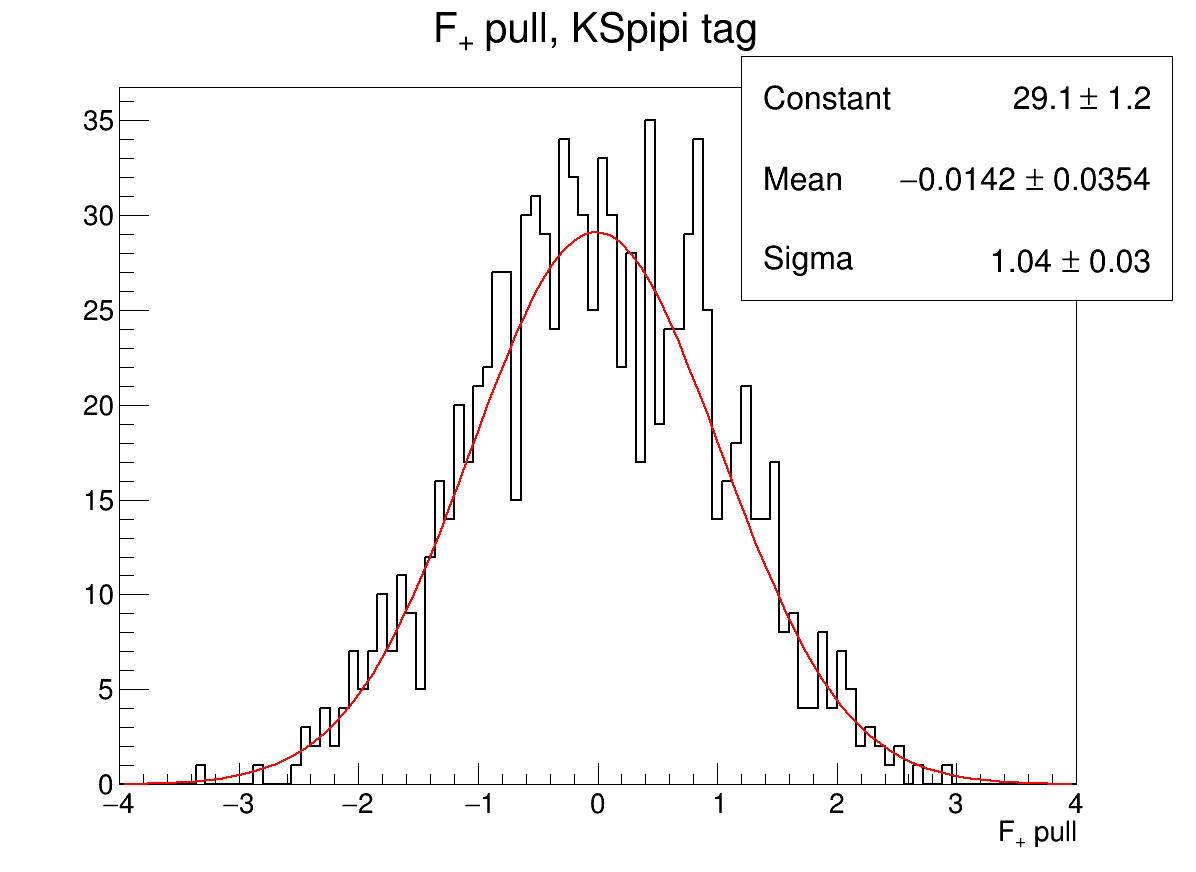
\includegraphics[width=\textwidth]{Plots/FPlus_toy_KSpipi.png}
      \caption{$K_S\pi\pi$ tag}
    \end{subfigure}%
    \begin{subfigure}{0.33\textwidth}
      \centering
      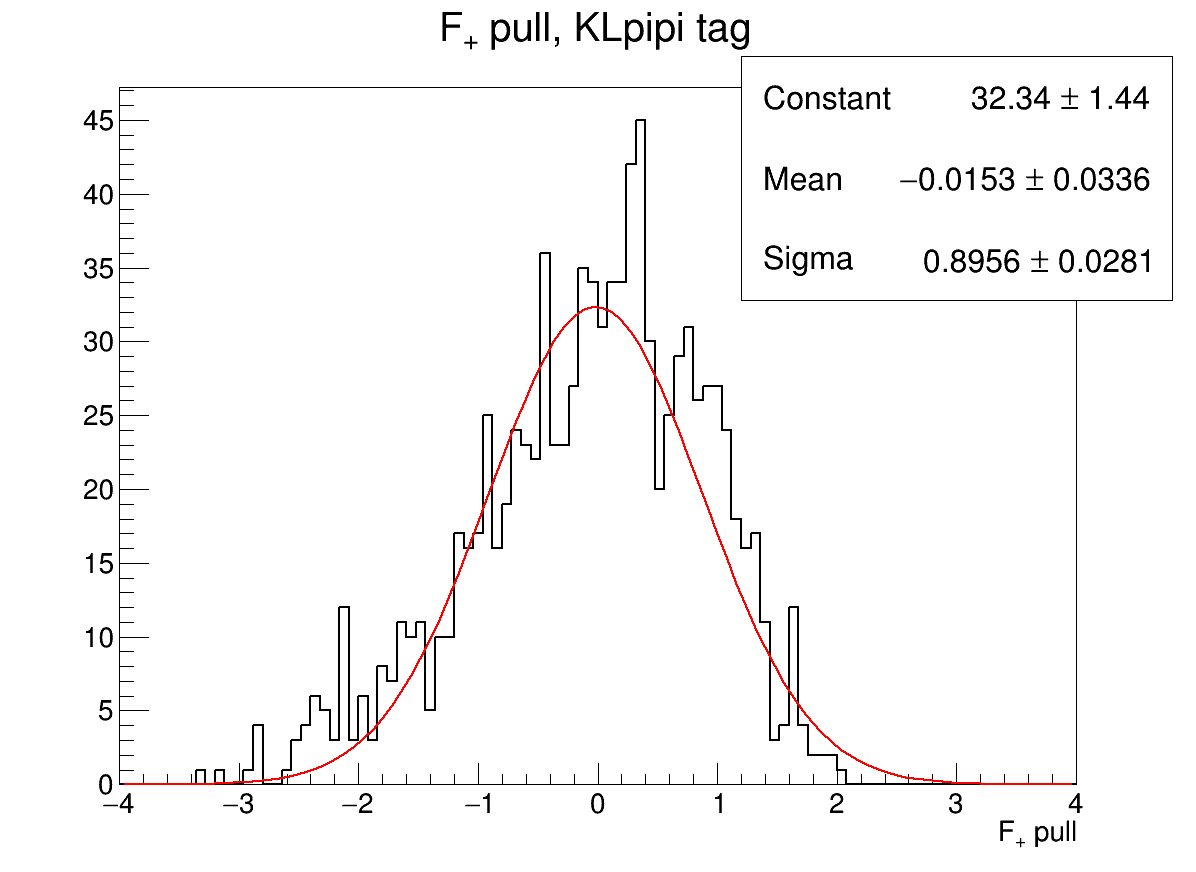
\includegraphics[width=\textwidth]{Plots/FPlus_toy_KLpipi.png}
      \caption{$K_L\pi\pi$ tag}
    \end{subfigure}
    \caption{$F_+$ pull distributions}
  \end{figure}
\end{frame}

\begin{frame}{Final fit results}
  \begin{figure}
    \centering
    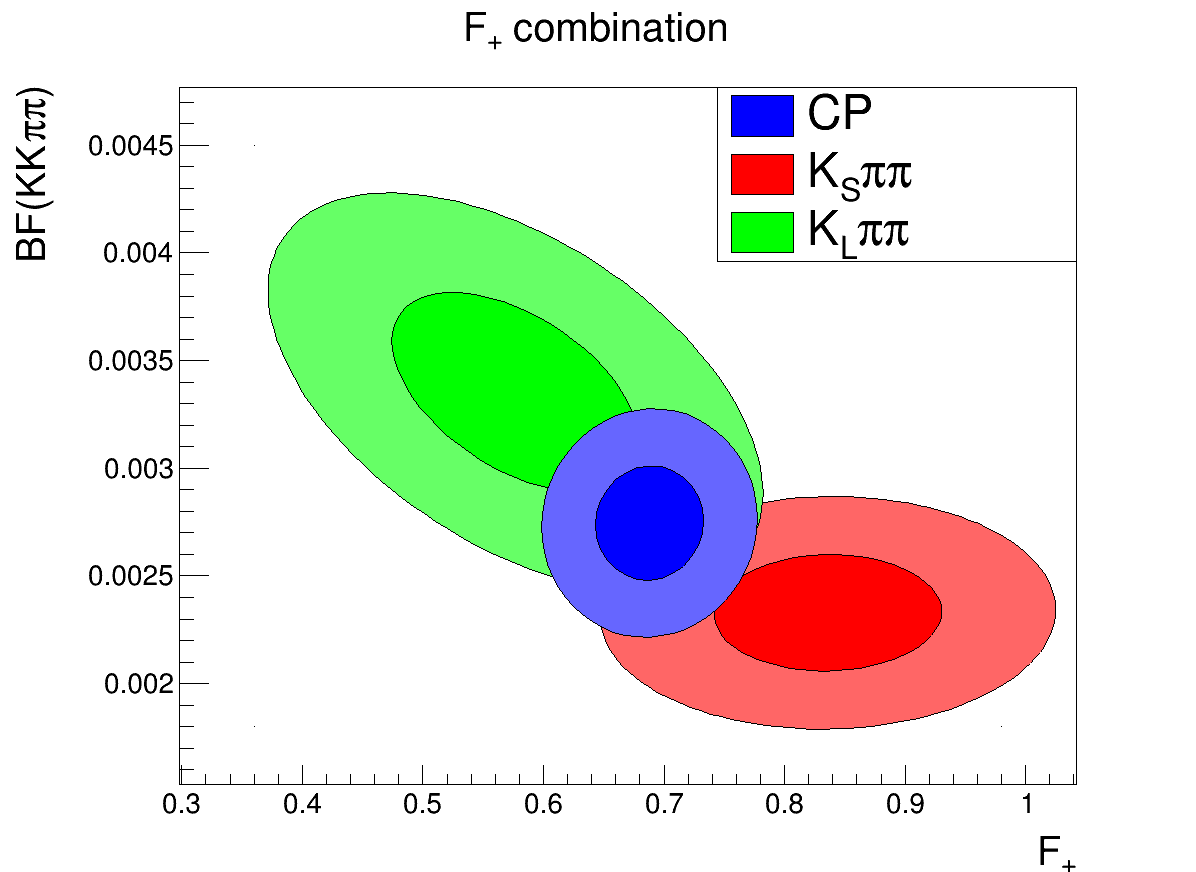
\includegraphics[width=0.7\textwidth]{Plots/FPlus_contours.png}
  \end{figure}
  \begin{itemize}
    \item{$K_L\pi\pi$ normalisation reduced by $14\%$ because of larger BF}
    \item{$K_L\pi\pi$ is potentially biased towards low $F_+$}
    \item{Only statistical uncertainties are shown}
  \end{itemize}
\end{frame}

\begin{frame}{Systematic uncertainties}
  \begin{enumerate}
    \item{External parameters: $F_+^{\pi\pi\pi^0}$, $c_i^{(\prime)}$, $K_i^{(\prime)}$}
    \begin{itemize}
      \item{Do a fit with these Gaussian constrained and subtract in quadrature}
      \item{Correlations between $c_i^{(\prime)}$ are accounted for}
    \end{itemize}
    \item{Peaking backgrounds}
    \begin{itemize}
      \item{Perform multiple fits to data with peaking background yields smeared}
      \item{In binned $K_{S, L}\pi\pi$, correlations are accounted for}
    \end{itemize}
    \item{Uncertainties in the efficiencies (finite MC samples)}
    \begin{itemize}
      \item{Multiple fits with smearing}
    \end{itemize}
    \item{$K_L\pi^0$ single tag yield}
    \begin{itemize}
      \item{Uncertainty from $K_L\pi^0$ BF and $N_{DD}$}
      \item{Smear ST yield and perform multiple fits}
    \end{itemize}
    \item{Efficiency factorisation}
    \begin{itemize}
      \item{Perform fit with DT efficiencies replaced by product of ST effiencies and take difference as a systematic}
    \end{itemize}
    \item{$K_S$ veto}
    \begin{itemize}
      \item{Calculate $F_+$ from model with and without $K_S$ veto and take the difference as a systematic}
    \end{itemize}
  \end{enumerate}
\end{frame}

\begin{frame}{Summary of all systematic uncertainties}
  \vspace{-0.3cm}
  \begin{center}
    Sources of $F_+$ systematics in units of $10^{-2}$ \\
    In addition, there is a $0.8\times 10^{-2}$ uncertainty from $K_S$ veto
  \end{center}
  \vspace{0.02cm}
  \begin{tabular}{lcccc} 
        \hline
        Source                   & CP tags                  & $K_{S, L}\pi\pi$ tags    & $K_S\pi\pi$ tag          & $K_L\pi\pi$ tag          \\
        \hline
        Statistical              & $4.5$                    & $8.3$                    & $8.4$                    & $10.3$                   \\
        \hline
        Efficiency               & $0.1$                    & $0.4$                    & $0.4$                    & $0.4$                    \\
        Efficiency factorisation & $0.6$                    & N/A                      & N/A                      & N/A                      \\
        External inputs          & $0.3$                    & $0.8$                    & $0.8$                    & $0.8$                    \\
        $K^0_L\pi^0$ ST yield    & $2.1$                    & N/A                      & N/A                      & N/A                      \\
        Peaking backgrounds      & $0.3$                    & $1.0$                    & $0.4$                    & $1.8$                    \\
        \hline
        Total                    & $2.2$                    & $1.3$                    & $1.0$                    & $2.0$                    \\
        \hline
  \end{tabular}
\end{frame}

\begin{frame}{Summary and conclusion}
  \begin{itemize}
    \setlength\itemsep{2.0em}
    \item{Finally finished with:}
    \begin{enumerate}
      \item{Peaking backgrounds}
      \item{Toy studies}
      \item{Reweighting}
      \item{Systematics}
    \end{enumerate}
    \item{Final result: $F_+ = 0.70 \pm 0.04$}
    \item{First draft of MEMO is finished and (hopefully) ready for circulation}
  \end{itemize}
\end{frame}

\end{document}